\chapter{Систення інформація за допомогою бінарних дерев}

\nopagebreak[4]
\section{Вступ}
\nopagebreak[4]
Дерево~--- це структура даних, що представляє собою сукупність елементів і відносин, що утворюють ієрархічну структуру цих елементів (рис.~\ref{f:tree1}). Кожен елемент дерева називається вершиною (вузлом) дерева. Вершини дерева з'єднані спрямованими дугами, які називають гілками дерева. Початковий вузол дерева називають коренем дерева, йому відповідає нульовий рівень. Листям дерева називають вершини, в які входить одна гілка і не виходить жодної гілки.

Кожне дерево має такі властивості:
\begin{itemize}
\item існує вузол, в який не входить ні однієї дуги (корінь);
\item в кожну вершину, крім кореня, входить одна дуга.
\end{itemize}


Дерева особливо часто використовують на практиці при зображенні різних ієрархій.

\begin{figure}
\caption{Дерево}\label{f:tree1}
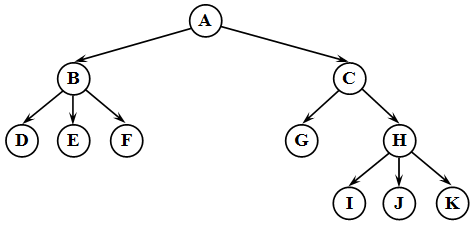
\includegraphics[width=13cm]{pic/31_01.png}

\end{figure}

Алгоритм Хаффмана - адаптивний жадний алгоритм оптимального префіксного кодування алфавіту з мінімальною надмірністю. Був розроблений в 1952 році аспірантом Массачусетського технологічного інституту Девідом Хаффманом при написанні їм курсової роботи. В даний час використовується в багатьох програмах стиснення даних.


\section{Ключові терміни}
\nopagebreak[4]

\textbf{Стиснення даних} - це процес, що забезпечує зменшення обсягу даних шляхом скорочення їх надмірності.

\textbf{Стиснення без втрат (повністю оборотне)} - це метод стиснення даних, при якому раніше закодована порція даних відновлюється після їх розпакування повністю без внесення змін.

\textbf{Стиснення з втратами} - це метод стиснення даних, при якому для забезпечення максимального ступеня стиску вихідного масиву даних частину містяться в ньому даних відкидається.

\textbf{Алгоритм стиснення даних (алгоритм архівації}) - це алгоритм, який усуває надмірність запису даних.

\textbf{Алфавіт коду} - це множина всіх символів вхідного потоку.

\textbf{Кодовий символ} - це найменша одиниця даних, що підлягає стисненню.

\textbf{Кодове слово} - це послідовність кодових символів з алфавіту коду.

\textbf{Токен} - це одиниця даних, записувана в стислий потік деяким алгоритмом стиснення.

\textbf{Фраза} - це фрагмент даних, що поміщається в словник для подальшого використання в стисненні.

\textbf{Кодування} - це процес стиснення даних.

\textbf{Декодування} - це зворотний кодуванню процес, при якому здійснюється відновлення даних.

\textbf{Ставлення стиснення} - це величина для позначення ефективності методу стиснення, що дорівнює відношенню розміру вихідного потоку до розміру вхідного потоку.

\textbf{Коефіцієнт стиснення} - це величина, зворотна відношенню стиснення.

\textbf{Середня довжина кодового слова} - це величина, яка обчислюється як зважена ймовірностями сума довжин всіх кодових слів.

\textbf{Статистичні методи} - це методи стиснення, що привласнюють коди змінної довжини символам вхідного потоку, причому більш короткі коди присвоюються символам або групам символам, що має більшу ймовірність появи у вхідному потоці.

\textbf{Словникове стиснення} - це методи стиснення, що зберігають фрагменти даних в деякій структурі даних, званої словником.

\textbf{Хаффманове кодування (стиснення)} - це метод стиснення, привласнює символам алфавіту коди змінної довжини грунтуючись на ймовірність появи цих символів.

\textbf{Префіксний код} - це код, в якому ніяке кодове слово не є префіксом будь-якого іншого кодового слова.

\textbf{Оптимальний префіксний код} - це префіксний код, що має мінімальну середню довжину.

\textbf{Кодова дерево (дерево кодування Хаффмана, Н-дерево)} - це бінарне дерево, у якого: листя позначені символами, для яких розробляється кодування; вузли (у тому числі корінь) позначені сумою ймовірностей появи всіх символів, відповідних листю поддерева, коренем якого є відповідний вузол.

\section{Розширені теоретичні відомості}
\nopagebreak[4]

\textbf{Кодова дерево (дерево кодування Хаффмана, Н-дерево)} - це бінарне дерево, у якого:

\begin{itemize}
\item листя позначені символами, для яких розробляється кодування;
\item вузли (у тому числі корінь) позначені сумою ймовірностей появи всіх символів, відповідних листю поддерева, коренем якого є відповідний вузол.,
\end{itemize}

Метод Хаффмана на вході отримує таблицю частот зустрічальності символів у вихідному тексті. Далі на підставі цієї таблиці будується дерево кодування Хаффмана.

Алгоритм побудови дерева Хаффмана.

\begin{enumerate}


\item Символи вхідного алфавіту утворюють список вільних вузлів. Кожен лист має вагу, що може бути дорівнює або ймовірності, або кількістю входжень символу в стискається текст.

\item Вибираються два вільні вузла дерева з найменшими вагами.

\item Створюється їх батько з вагою, рівним їх сумарному вазі.

\item Батько додається в список вільних вузлів, а двоє його дітей видаляються з цього списку.

\item Однією дузі, що виходить з батька, ставиться у відповідність біт 1, інший - біт 0.

\item Повторюємо кроки, починаючи з другого, до тих пір, поки в списку вільних вузлів не залишиться тільки один вільний вузол. Він і буде вважатися коренем дерева.
\end{enumerate}

Існує два підходи до побудови кодового дерева: від кореня до листя і від листя до кореня.

Приклад побудови кодового дерева. Нехай задана вихідна послідовність символів:

\verb'aabbbbbbbbccсcdeeeee'.

Її вихідний обсяг дорівнює 20 байт (160 біт). Згідно з наведеними на рис.~\ref{f:tree3} даними (таблиця ймовірності появи символів, кодове дерево і таблиця оптимальних префіксних кодів) закодована вихідна послідовність символів буде виглядати наступним чином:

\verb'110111010000000011111111111111001010101010'.

Отже, її обсяг буде дорівнює 42 біта. Коефіцієнт стиснення наближено дорівнює 3,8.
\begin{figure}
\caption{Дерево}\label{f:tree3}
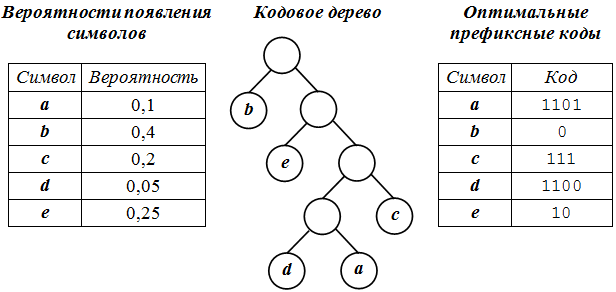
\includegraphics[width=13cm]{pic/41_01.png}

\end{figure}

Класичний алгоритм Хаффмана має один істотний недолік. Для відновлення вмісту стислого тексту при декодуванні необхідно знати таблицю частот яку використовували при кодуванні. Отже, довжина стислого тексту збільшується на довжину таблиці частот, яка повинна надсилатися попереду даних, що може звести нанівець всі зусилля зі стиснення даних. Крім того, необхідність наявності повної частотної статистики перед початком власне кодування вимагає двох проходів по тексту: одного для побудови моделі тексту (Таблиці частот і дерева Хаффмана), іншого для власне кодування.


У процесі роботи алгоритму стиснення вага вузлів в дереві кодування Хаффмана неухильно зростає. Перша проблема виникає тоді, коли вага кореня дерева починає перевершувати місткість комірки, в якій він зберігається. Як правило, це 16-бітове значення і, отже, не може бути більше, ніж 65535. Друга проблема, яка заслуговує ще більшої уваги, може виникнути значно раніше, коли розмір найдовшого коду Хаффмана перевершує місткість осередку, який використовується для того, щоб передати його у вихідний потік. Декодеру все одно, якої довжини код він декодує, оскільки він рухається зверху вниз по дереву кодування, вибираючи з вхідного потоку по одному біту. Кодер же повинен починати від листа дерева і рухатися вгору до кореня, збираючи біти, які потрібно передати. Зазвичай це відбувається зі змінною типу «ціле», і, коли довжина коду Хаффмана перевершує розмір типу «ціле» в бітах, настає переповнення.

\section{Приклади обчислень}
\nopagebreak[4]

Програмну реалізацію алгоритму надано у додатку \ref{code:haff}.





